\documentclass[12pt]{article}
\usepackage{amsfonts}
\usepackage{amsmath}
\usepackage{amssymb}
\usepackage{algorithm}
\usepackage{tikz}
\usetikzlibrary{positioning, calc}
\usepackage{algpseudocode}
\usepackage[top=1in, bottom=1in, left=1in, right=1in]{geometry}


\begin{document}
\pagenumbering{gobble}
\begin{center}
\textbf{Euklidischer Algorithmus\\}
\textbf{Proseminar Informatik ``Algorithms Unplugged''}\\
am Institut f\"ur Theoretische Informatik\\
Leibniz Universit\"at Hannover\\
\end{center}
\begin{flushright}
\textit{Bharat Ahuja\\Wintersemester 2014/15}
\end{flushright}

\noindent\makebox[\linewidth]{\rule{\paperwidth}{0.4pt}}
\vspace{10pt}
\begin{itemize}
	\item  Der euklidische Algorithmus ist ein Algorithmus, mit dem sich der \underline{gr\"o{\ss}te gemeinsame Teiler} (\textit{g.g.T.}) zweier nat\"urlicher Zahlen berechnen l\"asst. 
	\item Diesen Algorithmus hat Euklid ca. 300 \textit{v.Chr.} in \textit{Buch VII -- Die Elemente} (Proposition 1 und 2) als einen geometrischen Algorithmus vorgestellt.
	\item Berechnung von \textit{g.g.T.} relevant bei Gruppierung von Objekten, Pr\"ufen von Teilerfremdheit.
 
	\item Die Teilerfremdheit zweier Zahlen kann man alternativ durch das Vergleichen der Primfaktoren \"uberpr\"ufen.
	$$ggT(a,b) = \prod_{i \in \mathbb{N}} p_{i}^{min(a_i,b_i)}$$
	\item Die Bestimmung der Primfaktorzerlegung einer Zahl liegt aber in NP.
	\item \textsc{LangsamEuklid}\\\begin{algorithmic}[1]
\While {$a\neq b$}
	\State Falls $a$ gr\"o{\ss}er ist als $b, a\gets a-b$
	\State Falls $b$ gr\"o{\ss}er ist als $a, b\gets b-a$
\EndWhile
	\State Gib den gemeinsamen Wert der Zahlen aus
\end{algorithmic}
\vspace{10pt}
\begin{center}
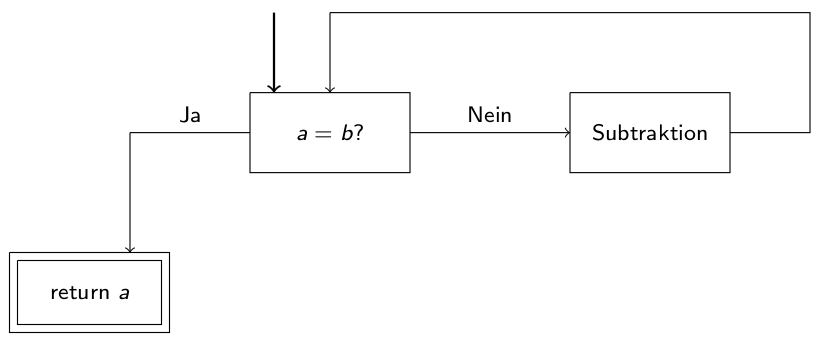
\includegraphics[scale=0.4]{langsamEuklid}
\end{center}
\newpage
	\item \textsc{Euklid} \\ \begin{algorithmic}[1]
		\State \textbf{if} $a < b$: vertausche a und b.
		\While {$b>0$}
		\State berechne $q,r$ mit $a=q\cdot b+r$, wobei $0\leq r < b$
		\State $a\gets b, b\gets r$
		\EndWhile
		\State \textbf{return} $a$
	\end{algorithmic}	
	\begin{center}
	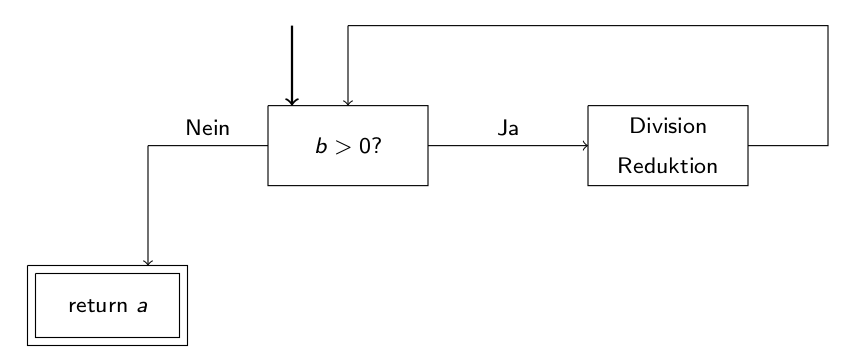
\includegraphics[scale=0.45]{euklid}
	\end{center}
	\vspace{10pt}
	\item \textsc{Euklid} effizienter als \textsc{LangsamEuklid} wegen Zusammenfassung mehrfacher Subtraktionen.
	\item Je schneller die Reste fallen, desto fr\"uher terminiert der Algorithmus. Die Fibonacci-Zahlen bilden den ung\"unstigsten Fall f\"ur diesen Algorithmus, weil alle Quotienten den kleinstm\"oglichen Wert annehmen, und dadurch die Reste sehr langsam fallen.
	\item Nach der ersten Iteration ist immer nur der Divisionsrest relevant.
	$$\therefore T_{b} = \frac{1}{b} \sum_{0 < k\leq b} T(k,b)$$
	\item Wenn man eine zuf\"allig gew\"ahlte Zahl auf Teilerfremdheit mit 5 pr\"ufen m\"ochte, braucht man im Schnitt $T_5=$ 2,6 Iterationen. Es gilt,
	$$T_n \approx \ln{n} + O(1)$$
\end{itemize}

\end{document}